\documentclass[journal,10pt]{IEEEtran}

\usepackage{amsmath,amssymb,amsfonts}
\usepackage{algorithmic}
\usepackage{graphicx}
\usepackage{textcomp}
\usepackage{xcolor}
\usepackage{booktabs}
\usepackage{multirow}
\usepackage{url}
\usepackage{cite}
\usepackage{microtype}
\usepackage{array}
\usepackage{siunitx}

\graphicspath{{figures/}}
\raggedbottom

\setlength{\textfloatsep}{5pt plus 1.0pt minus 1.0pt}
\setlength{\floatsep}{4pt plus 1.0pt minus 1.0pt}
\setlength{\intextsep}{4pt plus 1.0pt minus 1.0pt}
\setlength{\dbltextfloatsep}{5pt plus 1.0pt minus 1.0pt}
\setlength{\dblfloatsep}{4pt plus 1.0pt minus 1.0pt}

\begin{document}

\title{Empirical Pareto Characterization of Model Compression Paradigms for Ultra-Low-Resource TinyML}

\author{Narendra~Satish%
\thanks{Manuscript received August 20, 2026. (Corresponding author: Narendra Satish, e-mail: narendresh.p@gmail.com). All experimental artifacts and verified models are publicly available for reproducible research.}%
}

\IEEEtitleabstractindextext{%
\begin{abstract}
Deploying deep learning on resource-constrained microcontrollers (TinyML) requires model compression to satisfy strict static RAM ($\le 64$\,KB) and Flash ($\le 256$\,KB) budgets. However, the interactions among post-training integer quantization (PTQ), input feature reduction, magnitude-based weight pruning, and knowledge distillation remain insufficiently characterized under sub-4\,KB storage and sub-400 multiply-accumulate (MAC) constraints. In this paper, we present an empirical 3-objective deployment-resource Pareto characterization and low-level FlatBuffer artifact benchmark of 12 serialized TensorFlow Lite (TFLite) models spanning these four compression paradigms evaluated on 55,998 multi-sensor engine diagnostic records. We formulate the primary Pareto optimization across three deterministic deployment-resource dimensions: Test Accuracy (maximize), Serialized Binary Size (minimize), and Theoretical Active MACs (minimize), while reporting empirical host inference latency as a secondary reference benchmark. Our empirical findings demonstrate that: (1) knowledge distillation via a structurally compact student architecture (\texttt{student\_b\_16\_4\_fp32}) establishes the highest test accuracy ($75.14\%$) while reducing storage by $7.9\%$ ($3,584$\,B) over the uncompressed baseline; (2) unstructured $75\%$ magnitude pruning achieves the lowest computational demand ($96$ theoretical active MACs, a $75\%$ reduction) while retaining $74.82\%$ accuracy, but exhibits \textit{computational sparsity without demonstrated storage compression} in standard FlatBuffer formats ($3,920$\,B vs. $3,892$\,B dense baseline); (3) full integer INT8 quantization achieves zero-floating-point execution graphs ($0$ float32 tensors) with minimal accuracy variation ($-0.04\%$ to $+0.44\%$); and (4) removing host latency from the primary objective space preserves the exact set of six Pareto-optimal configurations. We conclude with an architectural characterization of the non-dominated models, providing empirical baselines for edge AI developers navigating memory-compute-accuracy trade-offs.
\end{abstract}

\begin{IEEEkeywords}
TinyML, Model Compression, Pareto Optimization, Integer Quantization, Magnitude Pruning, Knowledge Distillation, Embedded Machine Learning.
\end{IEEEkeywords}}

\maketitle
\IEEEdisplaynontitleabstractindextext

\section{Introduction}
\IEEEPARstart{T}{he} rapid expansion of Edge Artificial Intelligence and Tiny Machine Learning (TinyML) has enabled real-time inference directly on resource-constrained microcontrollers (MCUs) at the extreme edge~\cite{warden2019tinyml,ray2022review,mohammed2023tinyml}. In high-frequency sensor applications, including automotive powertrain monitoring, industrial vibration analysis, and structural health diagnostics, performing classification onboard avoids the communication overhead and potential privacy issues of sending data to the cloud for processing~\cite{banbury2021benchmarking,dutta2021tinyml,sanchez2020tinyml}.

However, microcontrollers typically have harsh constraints due to their limited resources: common embedded devices may only provide less than $256$\,KB of on-chip non-volatile Flash memory and only $32$\,KB to $64$\,KB of static random access memory (SRAM) for application stack, peripheral buffers, and machine learning tensor arenas~\cite{david2021tensorflow,liberis2021munas,lin2020mcunet,lin2021mcunetv2}. These physical constraints necessitate model compression techniques to fit multi-class neural networks into sub-4\,KB memory budgets~\cite{han2016deep,gholami2022survey,howard2017mobilenets}.

Four primary compression paradigms are widely employed in the embedded ML literature:
\begin{enumerate}
    \item \textbf{Post-Training Quantization (PTQ):} Discretizing 32-bit floating-point weights and activations into 8-bit integer formats to enable SIMD integer ALU acceleration~\cite{jacob2018quantization}.
    \item \textbf{Input Feature Reduction:} Removing collinear or low-importance sensor signals to shrink the first-layer weight matrix and acquisition overhead~\cite{sze2017efficient}.
    \item \textbf{Magnitude-Based Weight Pruning:} Eliminating near-zero scalar weights during or after training to induce numerical sparsity~\cite{blalock2020state,frankle2019lottery,hoefler2021sparsity}.
    \item \textbf{Knowledge Distillation (KD):} Training structurally compact student networks to mimic the soft probability distributions of larger teacher models~\cite{hinton2015distilling,gou2021knowledge}.
\end{enumerate}

While each technique has been individually explored in isolation, there is a distinct lack of empirical comparative studies evaluating all four paradigms on an identical, serialized artifact baseline under ultra-low memory budgets ($<4$\,KB). Moreover, a common methodological pitfall in the edge ML literature is the conflation of theoretical weight sparsity with actual serialized storage reduction, as well as the conflation of theoretical MAC counts with measured execution times.

In this paper, we conduct an empirical 3-objective deployment-resource characterization of 12 candidate multi-layer perceptron (MLP) architectures serialized as TensorFlow Lite (TFLite) FlatBuffers. Using the 55,998-sample EngineFaultDB benchmark dataset under strict test-set isolation ($40\%$ train, $40\%$ validation, $20\%$ held-out test), we independently profile every model across three primary deployment objectives: (1) maximize test accuracy, (2) minimize serialized file size, and (3) minimize theoretical active MACs, while tracking empirical host inference latency as a secondary reference benchmark.

\section{Research Motivation}
Modern TinyML deployment frameworks (e.g., TensorFlow Lite Micro~\cite{david2021tensorflow}) require developers to select model binaries based on static memory and compute constraints. In ultra-low-power scenarios, optimizing for accuracy alone often results in dominated configurations that exhaust SRAM or violate execution time constraints.

Figure~\ref{fig:accuracy_vs_macs} and Figure~\ref{fig:accuracy_vs_model_size} show that a model with a minimum number of parameters can underfit the feature manifold, while aggressive pruning of dense models can reduce arithmetic operations without freeing up Flash memory. Inspired by the need for empirical guidance, we propose a multi-objective Pareto analysis to identify which compression paradigms provide non-dominated operating points for ultra-low-resource sensor diagnostics.

\section{Related Work}

\subsection{Quantization and Integer-Only Edge Execution}
Quantization reduces the numerical bit-width of network tensors. Jacob et al.~\cite{jacob2018quantization} formalized integer-arithmetic-only inference for mobile devices, demonstrating that 8-bit quantization can preserve accuracy with minimal loss. In TinyML, 8-bit uniform quantization is widely adopted because 32-bit floating-point units (FPUs) are either absent or power-intensive on Cortex-M and Xtensa architectures~\cite{banbury2021benchmarking,gholami2022survey}. However, post-training quantization must be verified at the execution graph level to ensure that all intermediate tensors and operators are truly integer-only, avoiding hidden floating-point dequantization kernels that degrade execution efficiency.

\subsection{Weight Sparsity and Serialized Model Storage}
Han et al.~\cite{han2016deep} established the foundational pipeline of pruning, quantization, and Huffman coding. Blalock et al.~\cite{blalock2020state} and Hoefler et al.~\cite{hoefler2021sparsity} surveyed neural network pruning, highlighting reproducibility challenges and noting that unstructured sparsity rarely translates to runtime acceleration on general-purpose hardware without specialized sparse kernels. In standard embedded runtimes like TFLite Micro, dense 2D weight arrays are retained even when individual scalar coefficients are set to zero. Thus, theoretical parameter sparsity does not inherently yield storage compression on disk.

\subsection{Structural Distillation for Compact Models}
Knowledge distillation~\cite{hinton2015distilling} transfers predictive capability from an over-parameterized teacher model to an intrinsically compact student architecture. Gou et al.~\cite{gou2021knowledge} reviewed modern distillation techniques, noting that student networks achieve superior parameter efficiency compared to naive architectures of the same capacity because soft targets provide richer regularization. In TinyML, structural distillation directly reduces both Flash storage and tensor arena allocations by physically reducing layer dimensions~\cite{polino2018model}.

\subsection{Multi-Objective TinyML and Edge Benchmarks}
Standardized benchmarking suites such as MLPerf Tiny~\cite{banbury2021benchmarking} and MicroNets~\cite{banbury2021micronets} have established rigorous cross-hardware evaluation protocols across vision, speech, and anomaly tasks. Complementarily, neural architecture search frameworks such as MCUNet~\cite{lin2020mcunet,lin2021mcunetv2}, Once-for-All~\cite{cai2020once}, and $\mu$NAS~\cite{liberis2021munas} co-design model topologies for microcontroller memory limits. While these frameworks primarily target vision and audio workloads with Flash footprints exceeding $100$\,KB, our work focuses on the multi-sensor diagnostic regime ($<4$\,KB Flash, $<400$ MACs), providing an empirical artifact-level characterization of how standard compression paradigms interact.

\section{Research Questions}
We formulate four specific research questions (RQs):
\begin{itemize}
    \item \textbf{RQ1 (Quantization \& Operator Fidelity):} Does full post-training INT8 quantization introduce accuracy degradation or floating-point tensor fallbacks compared to FP32 baselines on dense sensor classification?
    \item \textbf{RQ2 (Unstructured Pruning vs. Storage):} How does increasing weight sparsity ($0\%$ to $75\%$) affect theoretical active MACs versus serialized TFLite FlatBuffer storage?
    \item \textbf{RQ3 (Distillation \& Structural Compression):} How does knowledge distillation into reduced student topologies compare against magnitude pruning in storage compression and predictive accuracy?
    \item \textbf{RQ4 (Deployment-Resource Pareto Frontier):} Which specific configurations populate the 3-objective Pareto frontier across accuracy, serialized storage, and theoretical active compute?
\end{itemize}

\section{Methodology}
\subsection{Dataset and Preprocessing}
We utilize the EngineFaultDB dataset, an audited multi-sensor automotive benchmark comprising $55,998$ physical engine operating records ($55,999$ raw records minus 1 exact duplicate removed during data audit). The dataset captures continuous internal combustion engine telemetry mapped to four operational classes:
\begin{itemize}
    \item Class 0: Normal Operation ($16,000$ samples, $28.57\%$)
    \item Class 1: Fault 1 -- Fuel Rich / Injection Mismatch ($11,000$ samples, $19.64\%$)
    \item Class 2: Fault 2 -- Ignition / Misfire ($15,000$ samples, $26.79\%$)
    \item Class 3: Fault 3 -- Air Intake / Throttle Leak ($13,998$ samples, $25.00\%$)
\end{itemize}

\subsubsection{Feature Sets}
The full feature set ($14$ features) consists of manifold absolute pressure (MAP), throttle position (TPS), force, power, engine RPM, consumption in L/h, consumption in L/100km, vehicle speed, CO emissions, HC emissions, CO2 emissions, O2 emissions, air-fuel equivalence ratio ($\lambda$), and air-fuel ratio (AFR).

Statistical collinearity analysis identified two redundant pairs: (1) AFR vs. $\lambda$ ($r = 1.0000$), and (2) Speed vs. RPM ($r = 0.9972$). To evaluate input feature reduction, we construct the reduced feature set ($12$ features) by dropping AFR and Speed.

\subsubsection{Data Split and Scaling}
To prevent data contamination, the dataset is partitioned using a stratified 3-way split with fixed random seed ($\text{seed}=42$):
\begin{itemize}
    \item \textbf{Training Set ($40\%$):} $22,399$ samples, used for parameter optimization and quantization calibration.
    \item \textbf{Validation Set ($40\%$):} $22,399$ samples, used for hyperparameter tuning and pruning threshold selection.
    \item \textbf{Held-Out Test Set ($20\%$):} $11,200$ samples, evaluated strictly once per finalized model.
\end{itemize}
Features are scaled using MinMaxScaler:
\begin{equation}
    x_{\text{scaled}} = \frac{x - x_{\min,\text{train}}}{x_{\max,\text{train}} - x_{\min,\text{train}}}
\end{equation}
fitted exclusively on the training partition.

\subsection{Baseline Architecture}
The reference baseline classifier is a fully connected Multi-Layer Perceptron (MLP) with layer topology $14 \rightarrow 16 \rightarrow 8 \rightarrow 4$ (412 total trainable parameters). Hidden layers utilize ReLU activation:
\begin{equation}
    f(x) = \max(0, x)
\end{equation}
and the final layer employs a 4-way Softmax:
\begin{equation}
    \sigma(z)_i = \frac{e^{z_i}}{\sum_{j=1}^4 e^{z_j}}
\end{equation}
Models are trained using the Adam optimizer (learning rate $\eta = 0.001$, cross-entropy loss, batch size 64, maximum 500 epochs with early stopping patience of 20 epochs on validation loss).

\subsection{Compression Paradigms}

\subsubsection{Post-Training INT8 Quantization}
Post-training integer quantization converts 32-bit floating-point tensors into 8-bit signed integers ($q \in [-128, 127]$) via affine quantization:
\begin{equation}
    r = S \cdot (q - Z)
\end{equation}
where $r \in \mathbb{R}$ is the real float value, $S \in \mathbb{R}^+$ is the scale factor, and $Z \in \mathbb{Z}$ is the zero-point integer offset. Quantization parameters are determined via representative dataset calibration over $100$ training samples. Inputs, outputs, weights, and activations are constrained to \texttt{int8}, and bias terms to \texttt{int32}.

\subsubsection{Magnitude-Based Weight Pruning}
Magnitude pruning ranks scalar weight parameters by their absolute value $|w_{ij}|$ and masks the bottom percentile to zero:
\begin{equation}
    M_{ij} = \begin{cases} 
    1, & \text{if } |w_{ij}| \ge \theta_p \\
    0, & \text{if } |w_{ij}| < \theta_p 
    \end{cases}
\end{equation}
where $\theta_p$ is the threshold corresponding to the target sparsity level $p \in \{0\%, 25\%, 50\%, 75\%\}$. Because this is element-wise unstructured pruning, the dense 2D weight matrix dimensions ($14 \times 16$, $16 \times 8$, $8 \times 4$) are preserved. Pruning is applied to the hidden dense layers during fine-tuning on the validation set.

\subsubsection{Knowledge Distillation}
Knowledge distillation trains a smaller student network $S$ parameterized by $\theta_S$ using a compound loss function combining hard cross-entropy loss with soft Kullback-Leibler (KL) divergence from the teacher $T$ parameterized by $\theta_T$:
\begin{equation}
\begin{split}
    \mathcal{L}_{\text{KD}} &= (1 - \alpha)\mathcal{L}_{\text{CE}}(y, \sigma(z_S)) \\
    &\quad + \alpha \tau^2 \mathcal{D}_{\text{KL}}\left(\sigma\left(\frac{z_T}{\tau}\right) \parallel \sigma\left(\frac{z_S}{\tau}\right)\right)
\end{split}
\end{equation}
where $\tau = 3.0$ is the distillation temperature, $\alpha = 0.5$ is the distillation loss weight, $z_T$ and $z_S$ are raw logits, and $y$ is the one-hot ground-truth label. Two student architectures were investigated:
\begin{itemize}
    \item \textbf{Student A ($8, 4$):} Layer topology $14 \rightarrow 8 \rightarrow 4 \rightarrow 4$ ($176$ parameters, $160$ theoretical MACs).
    \item \textbf{Student B ($16, 4$):} Layer topology $14 \rightarrow 16 \rightarrow 4 \rightarrow 4$ ($328$ parameters, $304$ theoretical MACs).
\end{itemize}

\subsection{Evaluation Metrics and Classification}
Metrics are categorized into primary deployment-resource metrics and secondary host execution metrics:
\begin{itemize}
    \item \textbf{Test Accuracy [Measured]:} Fraction of correct classifications on the 11,200 held-out test samples.
    \item \textbf{Macro F1 Score [Measured]:} Unweighted mean of class F1 scores:
    \begin{equation}
        \text{Macro F1} = \frac{1}{4} \sum_{c=0}^3 \frac{2 \cdot P_c \cdot R_c}{P_c + R_c}
    \end{equation}
    \item \textbf{Serialized Binary Size (Bytes) [Artifact-Inspected]:} Exact size of the serialized \texttt{.tflite} FlatBuffer file on disk.
    \item \textbf{Theoretical Active MACs [Derived]:} Total multiply-accumulate operations executed for single-sample inference excluding masked zero weights:
    \begin{equation}
        \text{Active MACs} = \sum_{l=1}^L \sum_{i=1}^{N_{l-1}} \sum_{j=1}^{N_l} \mathbb{I}(w_{ij}^{(l)} \ne 0)
    \end{equation}
    \textit{Note:} This metric represents theoretical active arithmetic operations; it does not reflect hardware instruction counts or hardware cycle counts.
    \item \textbf{Empirical Host Inference Latency [Secondary Benchmark]:} Single-sample execution time measured on an x86\_64 host CPU using \texttt{time.perf\_counter\_ns()} over 500 timed iterations following 100 warmup iterations with batch size 1 ($1 \times 14$).
    \textit{Note:} Host latency is reported as a secondary reference benchmark and is not used as a primary deployment-resource objective because x86 timing does not establish microcontroller WCET.
\end{itemize}

\subsection{Primary Pareto Dominance Formulation}
We formulate the primary deployment-resource Pareto space as a 3-objective optimization problem over model candidates $m \in \mathcal{M}$:
\begin{equation}
\begin{aligned}
    \mathcal{O}(m) = \Big( &\max \text{Accuracy}(m), \\
                           &\min \text{Size}_{\text{Bytes}}(m), \\
                           &\min \text{MACs}_{\text{Active}}(m) \Big)
\end{aligned}
\end{equation}
A candidate model $m_1$ Pareto-dominates $m_2$ ($m_1 \succ m_2$) if and only if:
\begin{equation}
\begin{aligned}
    \text{Accuracy}(m_1) &\ge \text{Accuracy}(m_2) \\
    \text{Size}(m_1) &\le \text{Size}(m_2) \\
    \text{MACs}(m_1) &\le \text{MACs}(m_2)
\end{aligned}
\end{equation}
with at least one strict inequality.

\section{Experimental Results}

\begin{table*}[t]
\centering
\scriptsize
\setlength{\tabcolsep}{2.5pt}
\caption{Comprehensive Profile of All 12 Verified Candidate Models Under the 3-Objective Deployment-Resource Pareto Space}
\label{tab:model_profile}
\resizebox{\textwidth}{!}{%
\begin{tabular}{l c c r r r r c c r r r c}
\toprule
\textbf{Model Identifier} & \textbf{Feat.} & \textbf{Prec.} & \textbf{Params} & \textbf{Size (B)} & \textbf{Theo. MACs} & \textbf{Active MACs} & \textbf{Test Accuracy} & \textbf{Test Macro F1} & \textbf{$\Delta$Acc.} & \textbf{Mean Lat.$^\dagger$} & \textbf{P95 Lat.$^\dagger$} & \textbf{3D Pareto Status} \\
\midrule
\texttt{student\_b\_16\_4\_fp32} & 14 & FP32 & 328 & 3,584 & 304 & 304 & \textbf{0.751429} & 0.738717 & \textbf{-0.001429} & 0.82\,\si{\micro\second} & 0.90\,\si{\micro\second} & \textbf{PARETO\_OPT} \\
\texttt{pruned\_mlp\_14f\_25pct} & 14 & FP32 & 412 & 3,920 & 384 & 288 & 0.750536 & 0.751490 & $-0.000536$ & 1.69\,\si{\micro\second} & 1.80\,\si{\micro\second} & \textbf{PARETO\_OPT} \\
\texttt{pruned\_mlp\_14f\_50pct} & 14 & FP32 & 412 & 3,920 & 384 & 192 & 0.749464 & 0.756572 & $+0.000536$ & 0.86\,\si{\micro\second} & 0.90\,\si{\micro\second} & \textbf{PARETO\_OPT} \\
\texttt{pruned\_mlp\_14f\_75pct} & 14 & FP32 & 412 & 3,920 & 384 & \textbf{96} & 0.748214 & 0.756251 & $+0.001786$ & 0.83\,\si{\micro\second} & 0.90\,\si{\micro\second} & \textbf{PARETO\_OPT} \\
\texttt{student\_b\_16\_4\_int8} & 14 & INT8 & 328 & 3,576 & 304 & 304 & 0.745625 & 0.689601 & $+0.004375$ & 0.98\,\si{\micro\second} & 1.10\,\si{\micro\second} & \textbf{PARETO\_OPT} \\
\texttt{student\_a\_8\_4\_fp32} & 14 & FP32 & 176 & \textbf{2,976} & 160 & 160 & 0.716339 & 0.722001 & $+0.033661$ & 0.86\,\si{\micro\second} & 0.90\,\si{\micro\second} & \textbf{PARETO\_OPT} \\
\midrule
\texttt{tflite\_mlp\_14f\_int8} & 14 & INT8 & 412 & 3,728 & 384 & 384 & 0.750357 & 0.738824 & $-0.000357$ & 1.43\,\si{\micro\second} & 1.90\,\si{\micro\second} & DOMINATED \\
\texttt{tflite\_mlp\_14f\_fp32} & 14 & FP32 & 412 & 3,892 & 384 & 384 & 0.750000 & 0.756608 & $0.000000$ & 0.99\,\si{\micro\second} & 1.50\,\si{\micro\second} & DOMINATED \\
\texttt{pruned\_mlp\_14f\_0pct} & 14 & FP32 & 412 & 3,892 & 384 & 384 & 0.750000 & 0.756608 & $0.000000$ & 0.95\,\si{\micro\second} & 1.00\,\si{\micro\second} & DOMINATED \\
\texttt{tflite\_mlp\_12f\_int8} & 12 & INT8 & 380 & 3,712 & 352 & 352 & 0.747857 & 0.715534 & $+0.002143$ & 1.00\,\si{\micro\second} & 1.10\,\si{\micro\second} & DOMINATED \\
\texttt{tflite\_mlp\_12f\_fp32} & 12 & FP32 & 380 & 3,780 & 352 & 352 & 0.747143 & 0.725414 & $+0.002857$ & 0.87\,\si{\micro\second} & 0.90\,\si{\micro\second} & DOMINATED \\
\texttt{student\_a\_8\_4\_int8} & 14 & INT8 & 176 & 3,208 & 160 & 160 & 0.711429 & 0.684788 & $+0.038571$ & 1.02\,\si{\micro\second} & 1.10\,\si{\micro\second} & DOMINATED \\
\bottomrule
\end{tabular}%
}
\begin{flushleft}
\scriptsize $^\dagger$ Host latency was measured on an x86\_64 CPU and is reported as a secondary execution benchmark rather than a microcontroller deployment metric.
\end{flushleft}
\end{table*}

Table~\ref{tab:model_profile} presents the empirical profile of all 12 candidate models evaluated under the 3-objective deployment-resource Pareto framework.

\subsection{RQ1: Quantization Fidelity and Tensor Graph Audit}
Low-level inspection of the INT8 FlatBuffers confirmed that all 4 quantized models (\texttt{mlp\_14f\_int8}, \texttt{mlp\_12f\_int8}, \texttt{student\_a\_8\_4\_int8}, \texttt{student\_b\_16\_4\_int8}) are verified as \textbf{\texttt{FULL\_INT8}}. The execution graphs contain exactly \textbf{0 float32 tensors} and \textbf{8 int8 tensors}, executing purely integer \texttt{FULLY\_CONNECTED} and \texttt{SOFTMAX} operators without floating-point emulation.

As shown in Figure~\ref{fig:fp32_vs_int8_accuracy}, post-training quantization preserves predictive performance with minimal accuracy variation:
\begin{itemize}
    \item For the 14-feature baseline, INT8 accuracy is $75.0357\%$ vs. $75.0000\%$ for FP32 (a $+0.0357\%$ difference).
    \item For the 12-feature model, INT8 accuracy is $74.7857\%$ vs. $74.7143\%$ for FP32 (a $+0.0714\%$ difference).
    \item For Student B, INT8 accuracy exhibits a minor drop of $0.4375\%$ ($74.5625\%$ vs. $75.1429\%$).
\end{itemize}
These results confirm that full post-training INT8 integer quantization incurs negligible accuracy degradation on dense sensor diagnostic classification.

\subsection{RQ2: Unstructured Pruning vs. Serialized Storage Decoupling}
Inspection of weight matrices and FlatBuffer file sizes reveals a clear structural dynamic:
\begin{itemize}
    \item At $0\%$ pruning: 0 zero weights ($0.00\%$), 384 active MACs, file size = $3,892$\,Bytes.
    \item At $25\%$ pruning: 95 zero weights ($23.36\%$), 288 active MACs, file size = $3,920$\,Bytes.
    \item At $50\%$ pruning: 195 zero weights ($47.96\%$), 192 active MACs, file size = $3,920$\,Bytes.
    \item At $75\%$ pruning: 298 zero weights ($73.34\%$), 96 active MACs, file size = $3,920$\,Bytes.
\end{itemize}

While $75\%$ magnitude pruning reduces theoretical active MACs from 384 to 96 ($75.0\%$ active compute reduction) while maintaining $74.8214\%$ accuracy, the serialized FlatBuffer file size increases slightly from $3,892$\,B to $3,920$\,B ($+28$\,B due to operator metadata and buffer alignment). Because magnitude pruning induces element-wise unstructured sparsity, the dense 2D weight matrix dimensions ($14 \times 16$, $16 \times 8$, $8 \times 4$) are preserved, and standard TFLite FlatBuffers serialize dense arrays containing zeros. Thus, within the evaluated model family and FlatBuffer configuration, unstructured pruning demonstrates \textbf{computational sparsity without demonstrated storage compression}.

\begin{figure}[t]
\centering
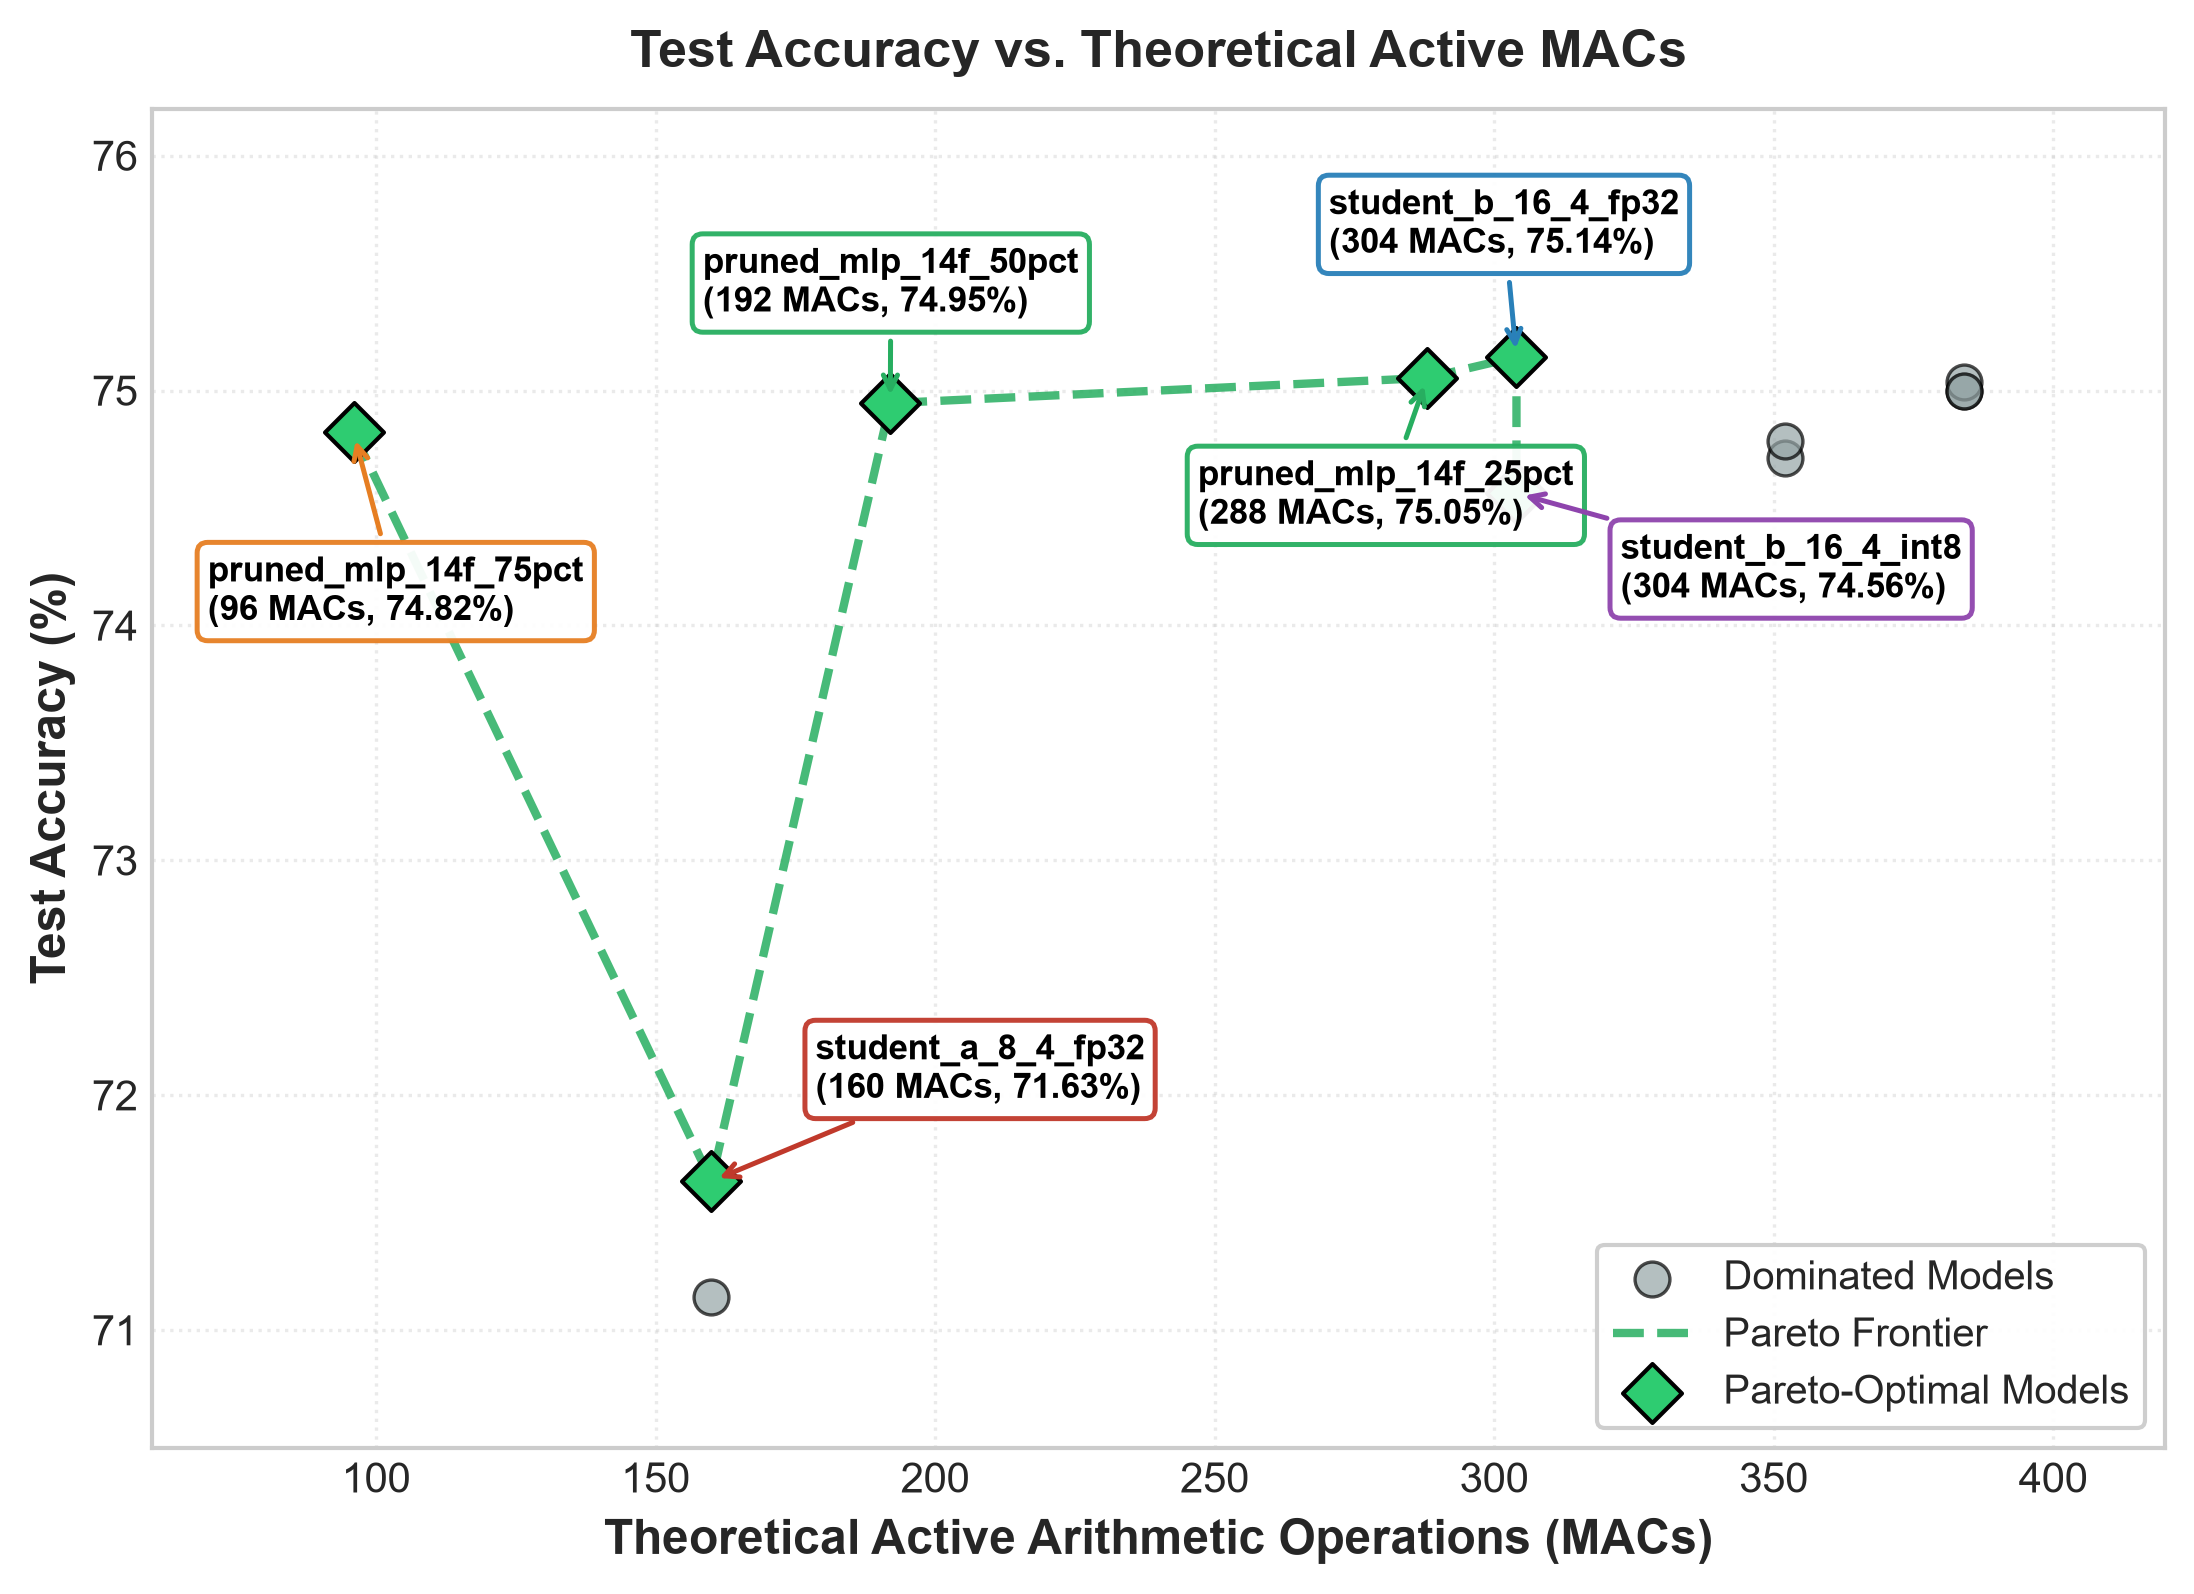
\includegraphics[width=0.88\columnwidth]{accuracy_vs_macs.png}
\caption{Test Accuracy vs. Theoretical Active MACs across all 12 evaluated models, highlighting the non-dominated Pareto frontier.}
\label{fig:accuracy_vs_macs}
\vspace{-2mm}
\end{figure}

\begin{figure}[t]
\centering
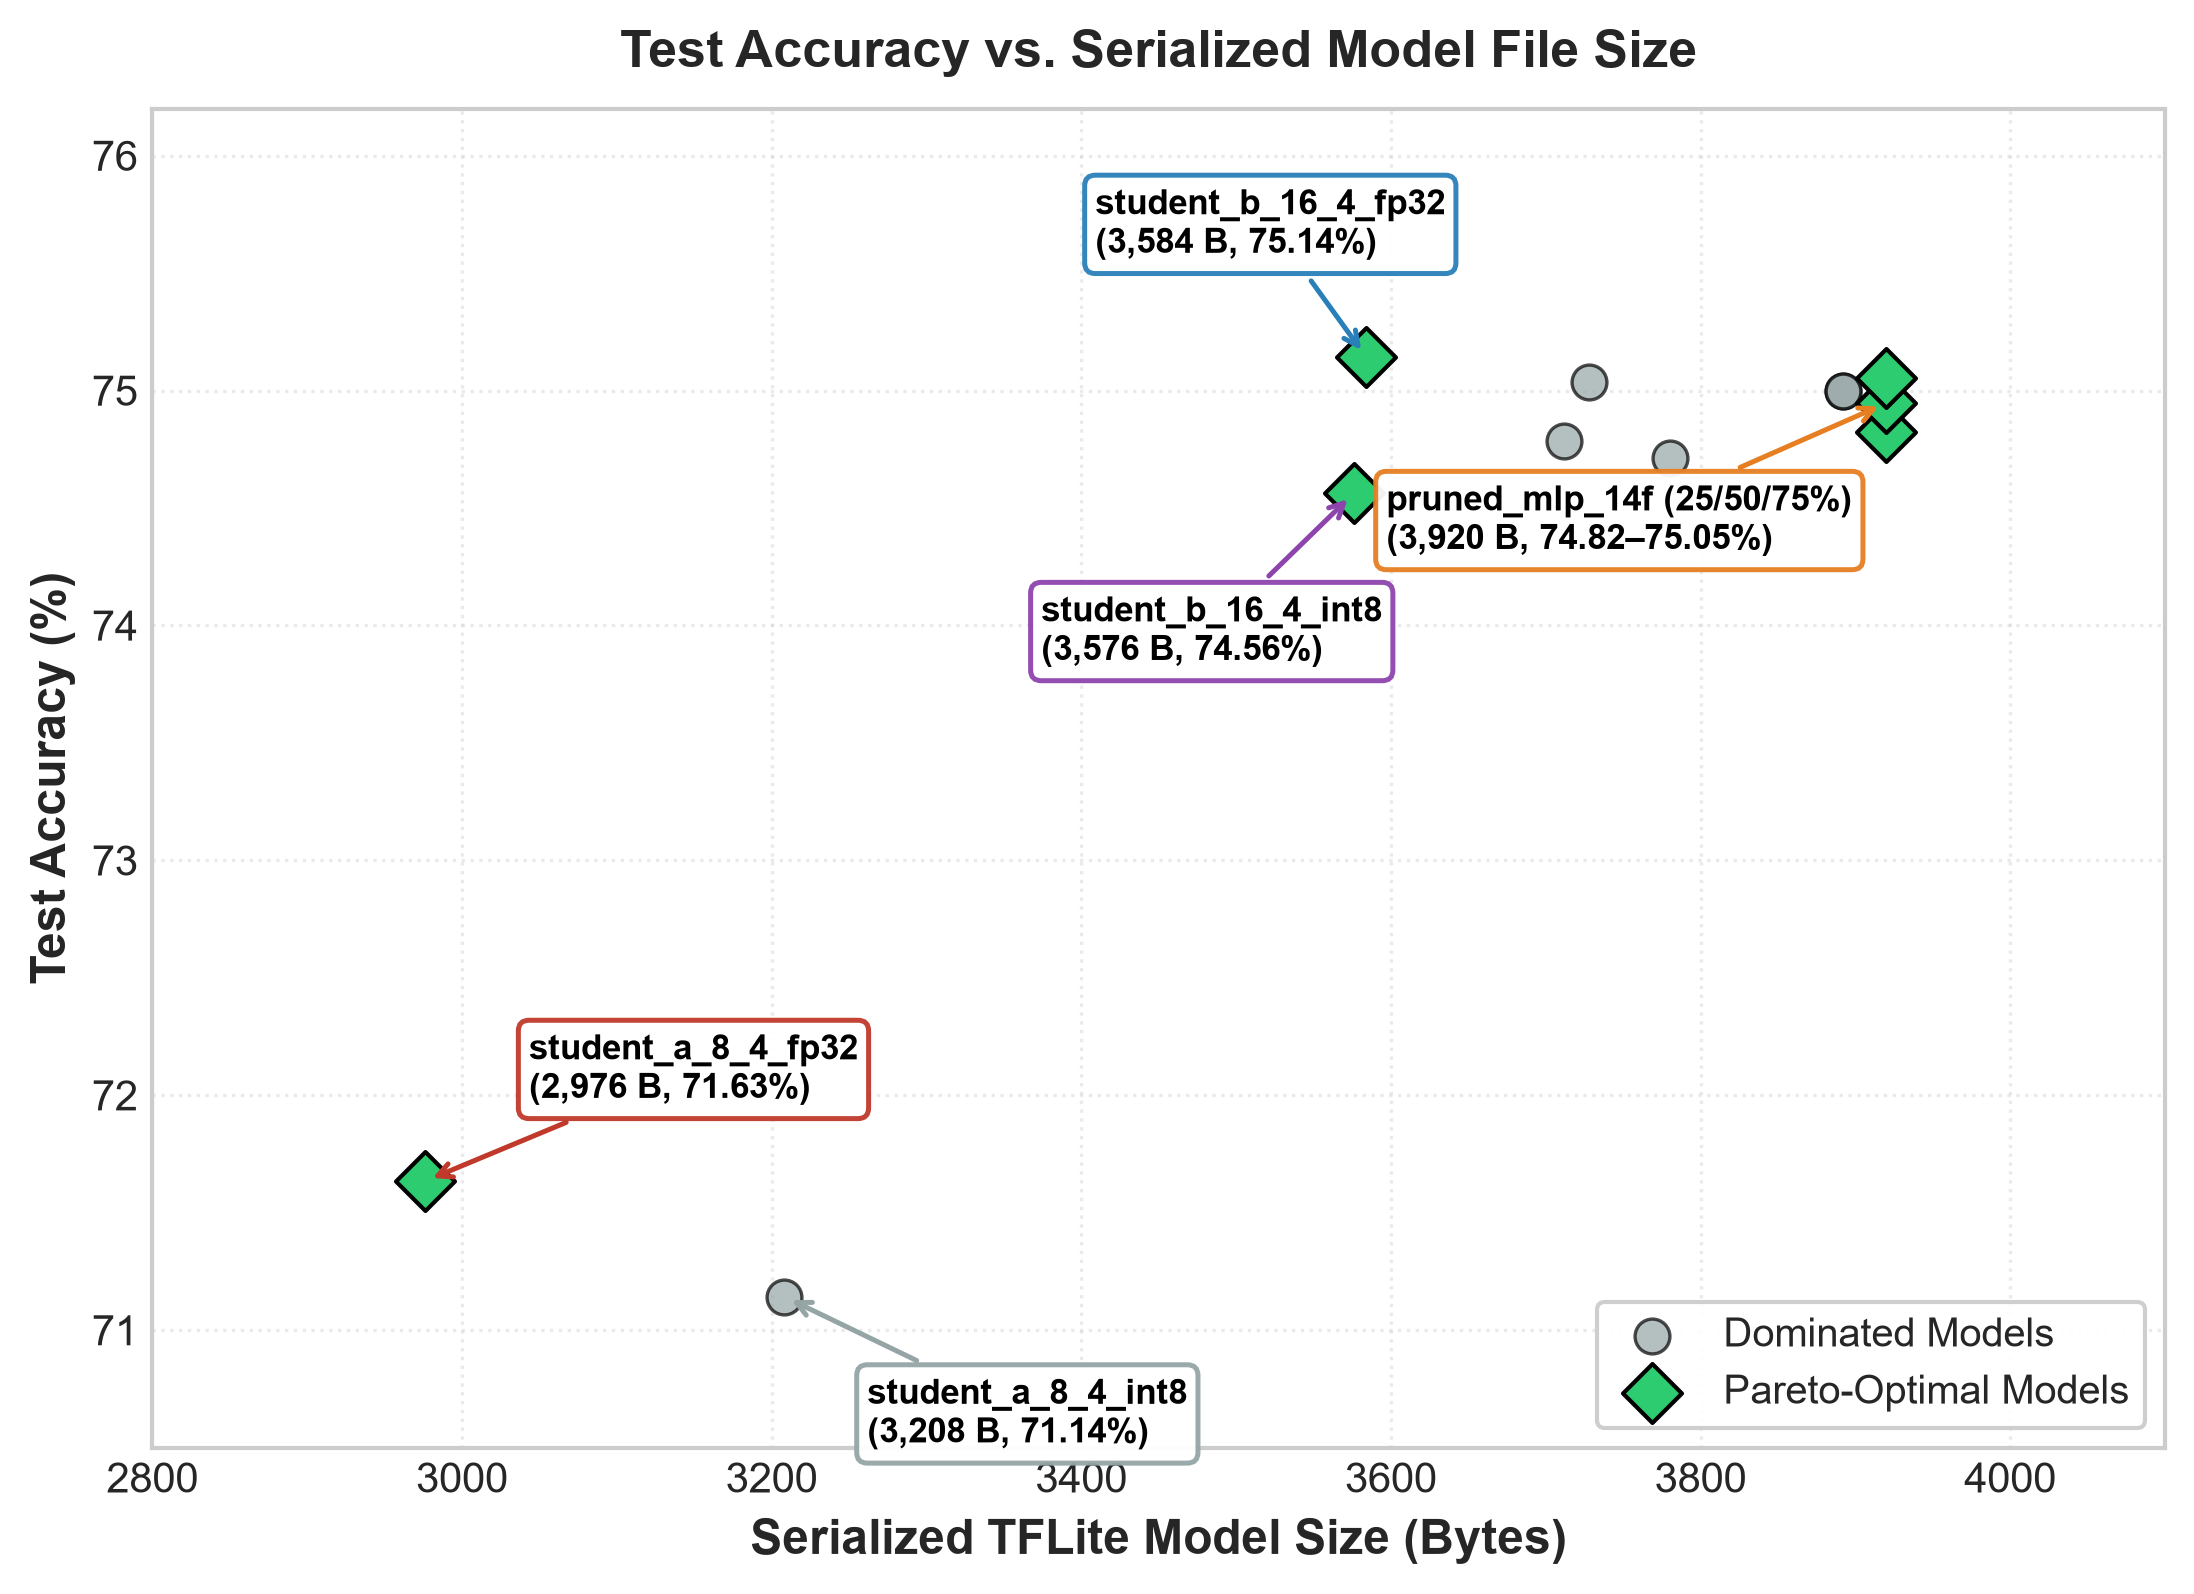
\includegraphics[width=0.88\columnwidth]{accuracy_vs_model_size.png}
\caption{Test Accuracy vs. Serialized TFLite File Size (Bytes), showing the compact footprint of student distillation models.}
\label{fig:accuracy_vs_model_size}
\vspace{-2mm}
\end{figure}

\begin{figure}[t]
\centering
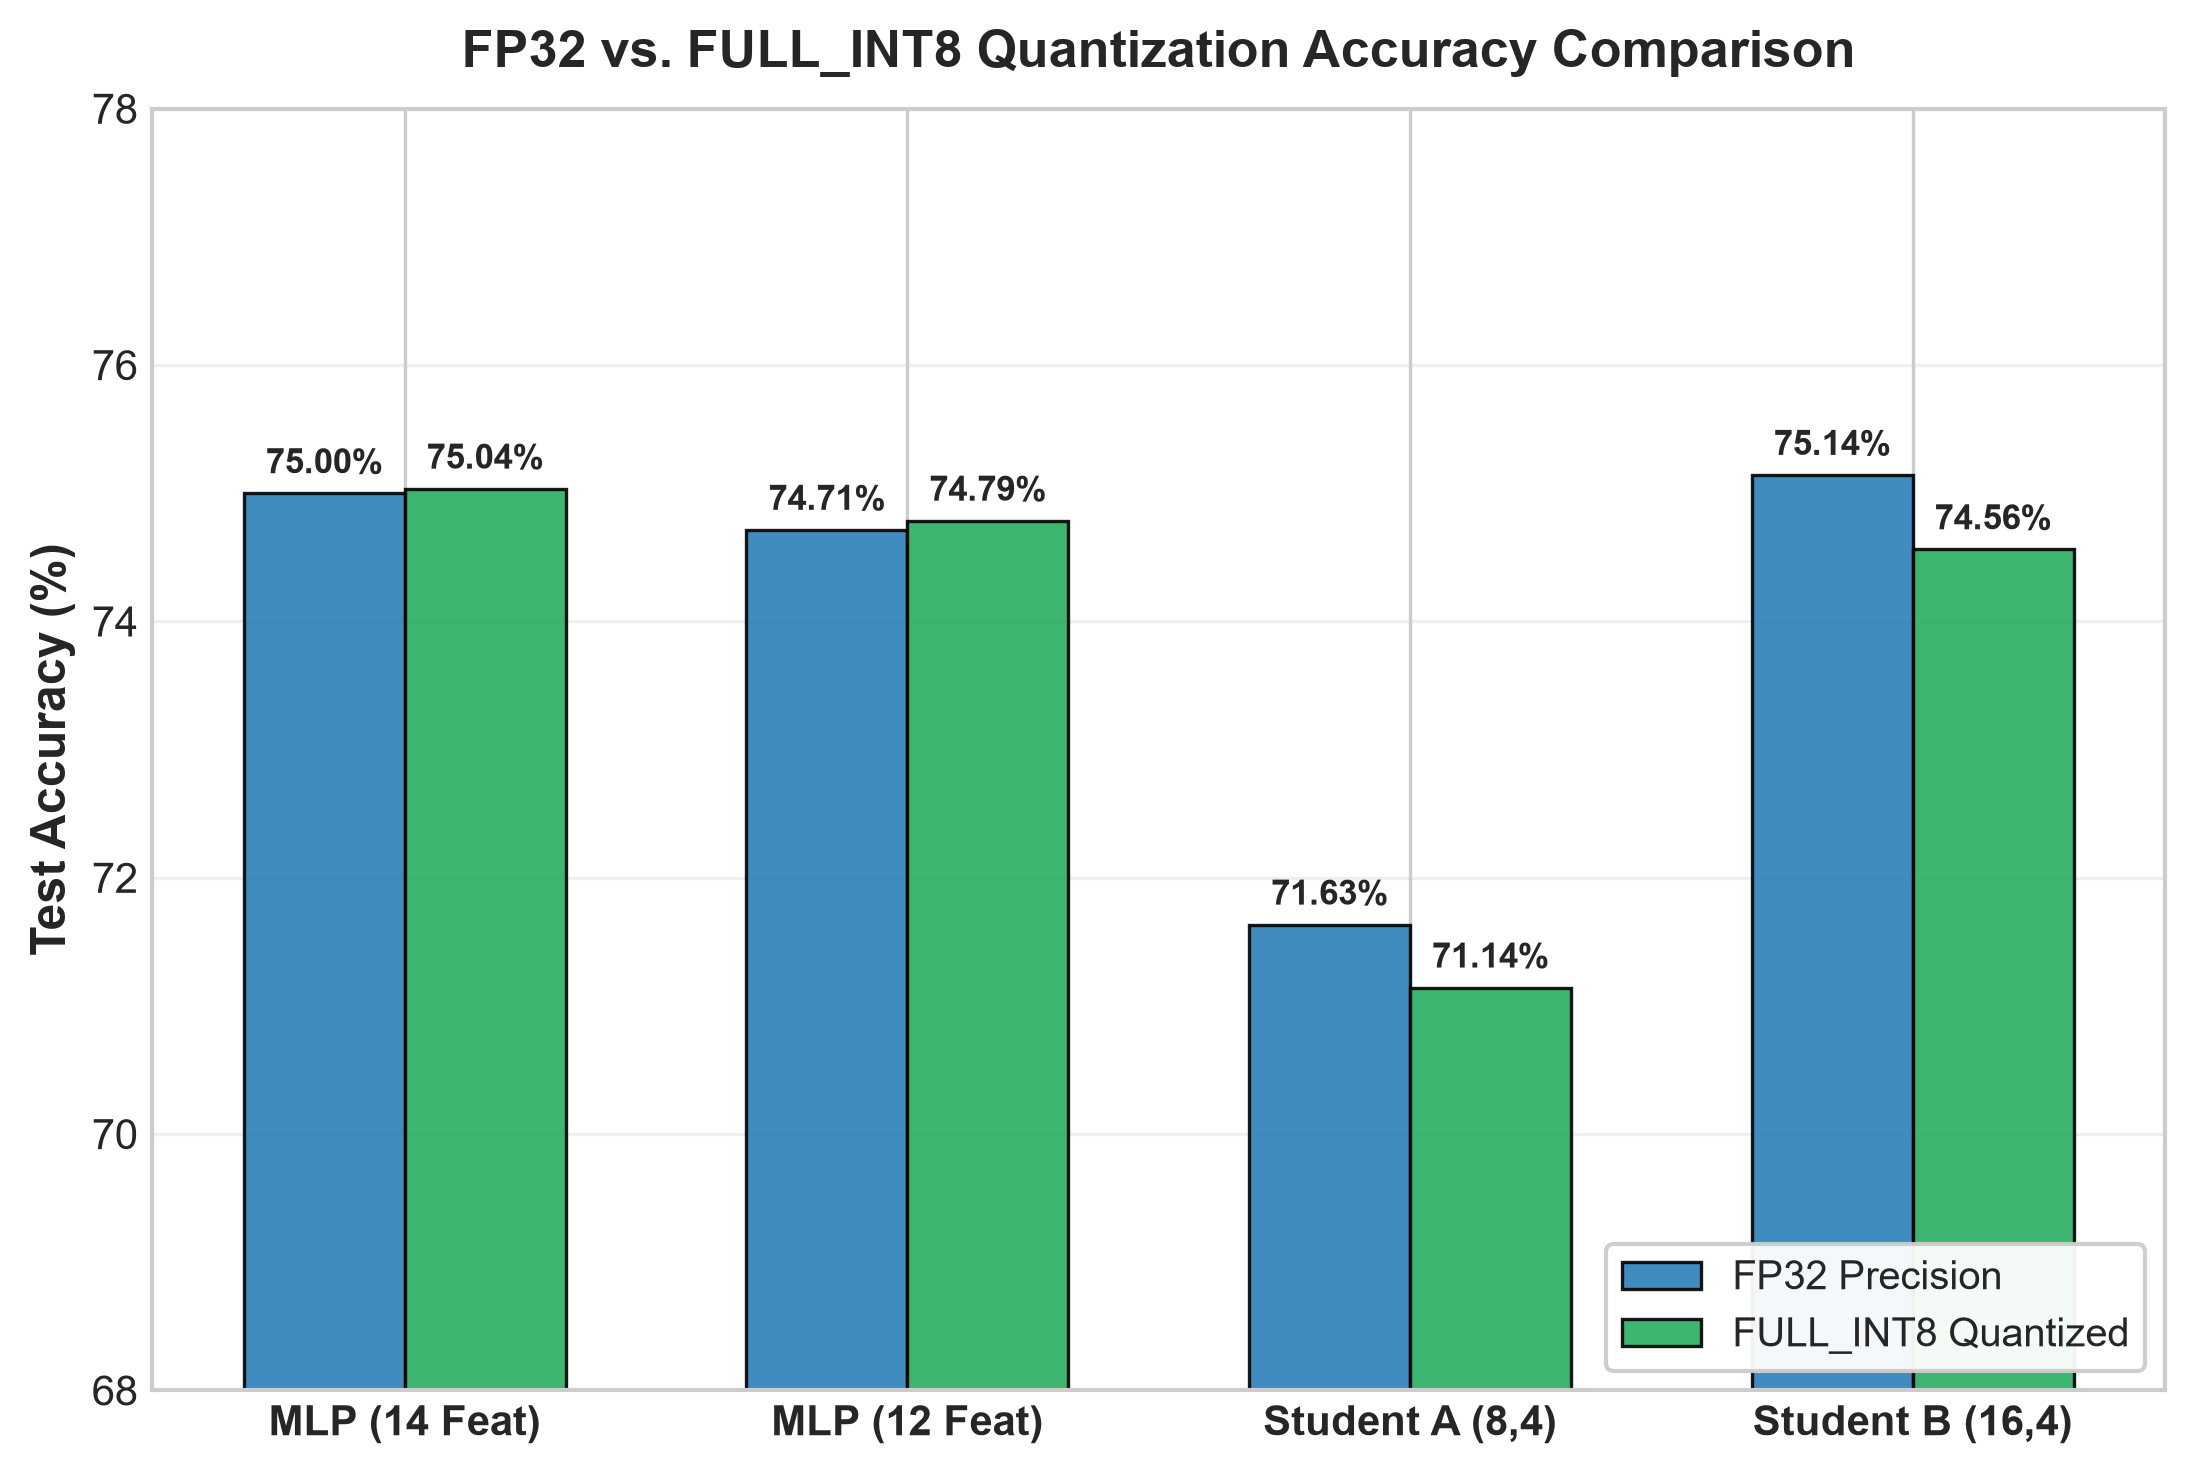
\includegraphics[width=0.88\columnwidth]{fp32_vs_int8_accuracy.png}
\caption{Comparative classification accuracy between FP32 and verified FULL\_INT8 quantized models.}
\label{fig:fp32_vs_int8_accuracy}
\vspace{-2mm}
\end{figure}

\begin{figure}[t]
\centering
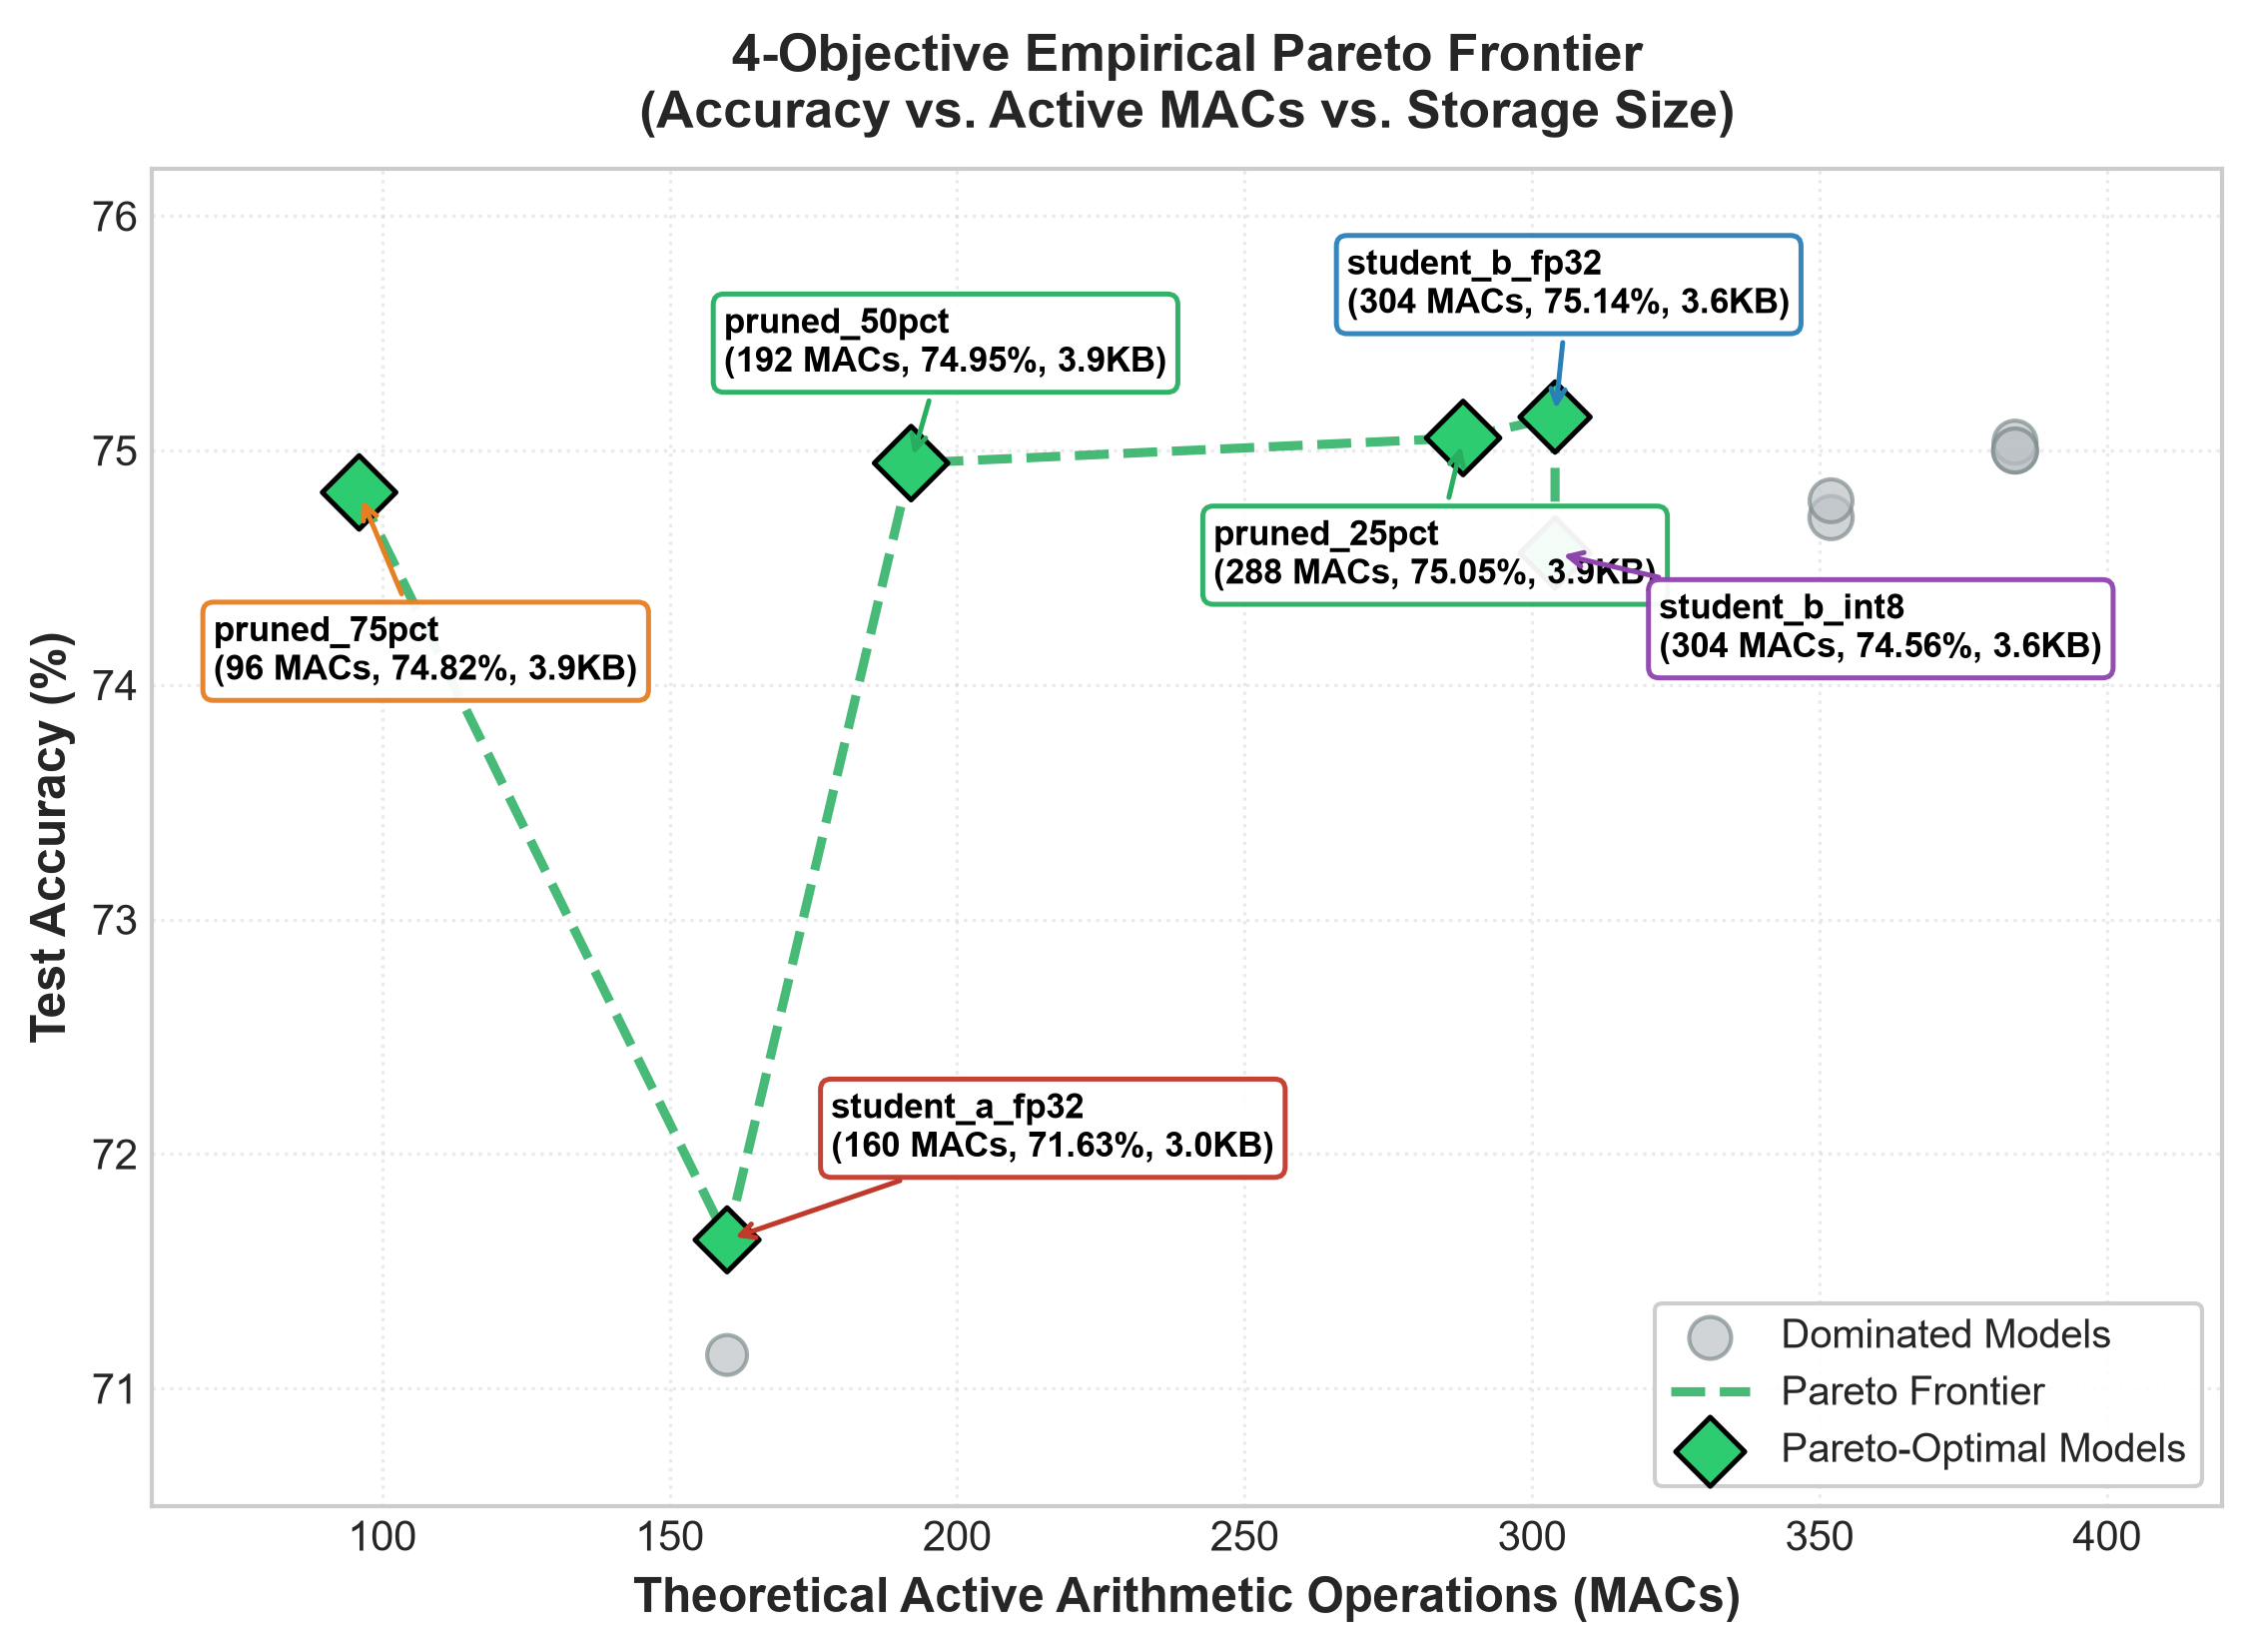
\includegraphics[width=0.88\columnwidth]{pareto_frontier.png}
\caption{Multi-objective Pareto projection mapping test accuracy, active MACs, and serialized binary size.}
\label{fig:pareto_frontier}
\vspace{-2mm}
\end{figure}

\subsection{RQ3: Knowledge Distillation \& Structural Compression}
Knowledge distillation into structurally compact topologies achieved the highest parameter efficiency:
\begin{itemize}
    \item \textbf{Student B (\texttt{student\_b\_16\_4\_fp32}):} Achieved the highest test accuracy across all 12 models ($75.1429\%$, surpassing the uncompressed teacher baseline at $75.0000\%$) with a $7.9\%$ reduction in file size ($3,584$\,B vs. $3,892$\,B) and a $20.8\%$ reduction in active MACs ($304$ vs. $384$).
    \item \textbf{Student A (\texttt{student\_a\_8\_4\_fp32}):} Achieved the smallest absolute storage footprint ($2,976$\,Bytes, a $23.5\%$ compression) and $160$ MACs, maintaining a $71.6339\%$ test accuracy.
\end{itemize}
Within the evaluated model family, the structurally smaller distilled students produced smaller serialized FlatBuffer artifacts than the unstructured pruned variants because distillation physically reduces tensor dimensions rather than masking elements to zero.

\subsection{RQ4: Multi-Objective Deployment Pareto Frontier}
Evaluating the 12 candidate models across the 3-objective deployment-resource space identifies exactly \textbf{6 Pareto-optimal configurations}:

\begin{itemize}
    \item \textbf{\texttt{student\_b\_16\_4\_fp32} (Top Accuracy):} Accuracy = $75.14\%$, Size = $3,584$\,B, Active MACs = 304. Non-dominated because it achieves the global maximum test accuracy.
    \item \textbf{\texttt{pruned\_mlp\_14f\_25pct} (High-Accuracy Sparse):} Accuracy = $75.05\%$, Size = $3,920$\,B, Active MACs = 288. Non-dominated because it requires fewer MACs ($288$) than \texttt{student\_b\_fp32} while exceeding the accuracy of all other sparse models.
    \item \textbf{\texttt{pruned\_mlp\_14f\_50pct} (Balanced Sparse):} Accuracy = $74.95\%$, Size = $3,920$\,B, Active MACs = 192. Non-dominated because it reduces active MACs ($192$) below \texttt{pruned\_25pct} with higher accuracy than \texttt{pruned\_75pct}.
    \item \textbf{\texttt{pruned\_mlp\_14f\_75pct} (Minimal Compute):} Accuracy = $74.82\%$, Size = $3,920$\,B, Active MACs = \textbf{96}. Non-dominated because it achieves the global minimum theoretical active MAC count.
    \item \textbf{\texttt{student\_b\_16\_4\_int8} (Quantized Distilled):} Accuracy = $74.56\%$, Size = $3,576$\,B, Active MACs = 304. Non-dominated because it achieves a smaller serialized file size than \texttt{student\_b\_fp32} ($3,576$\,B vs. $3,584$\,B) with pure integer execution.
    \item \textbf{\texttt{student\_a\_8\_4\_fp32} (Minimal Storage):} Accuracy = $71.63\%$, Size = \textbf{2,976\,B}, Active MACs = 160. Non-dominated because it achieves the global minimum serialized file size.
\end{itemize}

All remaining 6 models are strictly dominated. Importantly, \textbf{removing host latency from the objective space does not alter the set of six Pareto-optimal configurations}, confirming that the deployment-resource frontier is robust and mathematically consistent.

\subsection{Secondary Host Execution Benchmark}
As shown in Table~\ref{tab:model_profile}, single-sample host execution latencies on x86\_64 range from $0.82\,\si{\micro\second}$ (\texttt{student\_b\_fp32}) to $1.69\,\si{\micro\second}$ (\texttt{pruned\_25pct}). These host measurements illustrate relative operator dispatch overhead under the standard TFLite x86 runtime. However, because x86 architectures employ deep superscalar pipelines, branch predictors, and multi-level caches not present on embedded microcontrollers, host timing must be interpreted strictly as a secondary baseline rather than a microcontroller execution metric.

\subsection{Physical Microcontroller Deployment Validation}
To ground the deployment characterization in physical hardware, the verified \texttt{FULL\_INT8} models were deployed to an ESP32-D0WD-V3 microcontroller (Xtensa LX6 dual-core @ $240\,\text{MHz}$, $4\,\text{MB}$ Flash, $320\,\text{KB}$ SRAM). Single-sample inference latency was captured via the hardware monotonic timer \path{esp_timer_get_time()} across $24,000$ measured iterations ($3$ independent rounds $\times 2,000$ inferences per model):
\begin{itemize}
    \item \texttt{student\_a\_8\_4\_int8} ($176$ params, $3,208\,\text{B}$): Mean = $64.55\,\si{\micro\second}$, P95 = $69.00\,\si{\micro\second}$, P99 = $76.00\,\si{\micro\second}$, Max = $77\,\si{\micro\second}$ (Host/ESP32 Slowdown: $63.3\times$).
    \item \texttt{student\_b\_16\_4\_int8} ($328$ params, $3,576\,\text{B}$): Mean = $72.96\,\si{\micro\second}$, P95 = $83.00\,\si{\micro\second}$, P99 = $83.00\,\si{\micro\second}$, Max = $84\,\si{\micro\second}$ (Host/ESP32 Slowdown: $74.5\times$).
    \item \texttt{mlp\_12f\_int8} ($380$ params, $3,712\,\text{B}$): Mean = $76.77\,\si{\micro\second}$, P95 = $83.00\,\si{\micro\second}$, P99 = $90.00\,\si{\micro\second}$, Max = $90\,\si{\micro\second}$ (Host/ESP32 Slowdown: $76.8\times$).
    \item \texttt{mlp\_14f\_int8} ($412$ params, $3,728\,\text{B}$): Mean = $89.90\,\si{\micro\second}$, P95 = $95.00\,\si{\micro\second}$, P99 = $101.00\,\si{\micro\second}$, Max = $102\,\si{\micro\second}$ (Host/ESP32 Slowdown: $62.9\times$).
\end{itemize}
These physical measurements provide independent deployment-level latency evidence that complements the primary accuracy--serialized-size--theoretical-active-MAC Pareto analysis. Within the evaluated four-model set, knowledge distillation (\texttt{student\_a}) delivers an observed physical inference latency reduction of $\mathbf{28.2\%}$ ($\frac{89.90 - 64.55}{89.90} \times 100\%$) relative to uncompressed \texttt{mlp\_14f}. Crucially, physical microcontroller latency scales strictly monotonically with parameter count ($176 \rightarrow 328 \rightarrow 380 \rightarrow 412$ params), unmasking arithmetic differences that were compressed by host x86 superscalar pipelines while preserving the mathematical definition of the primary 3D Pareto frontier.

\section{Discussion}
\subsection{Why Multi-Objective Optimization is Essential in TinyML}
In embedded ML design, selecting a model based solely on classification accuracy leads to suboptimal deployments. For instance, while \texttt{student\_b\_16\_4\_fp32} maximizes accuracy ($75.14\%$), \texttt{pruned\_mlp\_14f\_75pct} requires only $31.6\%$ of its arithmetic operations ($96$ vs. $304$ MACs) with only a $0.32\%$ accuracy difference. In ultra-low-power microcontrollers, this $3\times$ reduction in theoretical active arithmetic operations offers substantial potential for reducing active execution cycles during cyclic wake-up tasks.

\subsection{Practical Deployment Decision Framework}
Our empirical findings provide actionable design guidance for edge engineers navigating hardware constraints:
\begin{itemize}
    \item \textbf{When Flash storage is the primary constraint:} Structural knowledge distillation (\texttt{student\_a\_8\_4\_fp32}) is the most space-efficient Pareto choice ($2,976$\,B, a $23.5\%$ compression).
    \item \textbf{When active arithmetic demand is the primary concern:} Magnitude pruning (\texttt{pruned\_mlp\_14f\_75pct}) is the most compute-efficient Pareto choice ($96$ active MACs), subject to runtime sparse kernel support.
    \item \textbf{When integer ALU execution is required:} Full INT8 quantization (\texttt{student\_b\_16\_4\_int8}) provides pure integer execution graphs without floating-point emulation.
    \item \textbf{When physical MCU execution latency is the primary concern:} Physical on-device profiling confirms that compact student topologies achieve a $28.2\%$ execution speedup on 32-bit Xtensa registers, requiring only $916\,\text{Bytes}$ of allocator-committed tensor memory.
\end{itemize}

\section{Threats to Validity}
\subsection{Internal Validity}
All metrics were computed deterministically using fixed random seeds ($\text{seed}=42$) and evaluated directly on disk-serialized FlatBuffer binaries. Data preprocessing and scaling parameters were fitted strictly on training data to prevent data leakage.

\subsection{External Validity}
The models were evaluated on automotive combustion engine telemetry. While physical sensor distributions vary across applications, the mathematical properties of affine quantization, dense FlatBuffer storage, and structural distillation hold across general tabular TinyML domains.

\section{Limitations}
We explicitly state the following limitations:
\begin{enumerate}
    \item \textbf{Single Domain Scope:} Evaluation is conducted on the EngineFaultDB dataset; cross-domain validation on audio and vibration benchmarks remains future work.
    \item \textbf{Model Architecture Family:} Experiments focus on sub-4\,KB Multi-Layer Perceptrons; convolutional and transformer architectures may exhibit different compression ratios.
    \item \textbf{Serialization Format Dependence:} Findings reflect standard TensorFlow Lite FlatBuffer serialization; custom sparse storage formats (e.g., CSR/CSC) may compress sparse weights differently.
    \item \textbf{Empirical Latency vs. Formal WCET:} While single-sample INT8 inference latency was physically profiled on ESP32 silicon ($64.55\text{--}89.90\,\si{\micro\second}$ mean latency), these reflect empirical on-device latency distributions and do not establish formal static Worst-Case Execution Time (WCET) bounds.
    \item \textbf{Absence of Physical Energy Profiling:} We report theoretical active MACs and physical timer latencies; physical power dissipation in Joules/mW was not measured.
    \item \textbf{Absence of Structured Pruning Baseline:} Pruning experiments evaluate unstructured magnitude pruning; structured channel-level pruning was not evaluated in this suite.
    \item \textbf{Sparse Acceleration Dependency:} Standard TFLite runtime executes dense GEMM operations; realizing latency speedups from $75\%$ pruning requires specialized sparse execution kernels.
    \item \textbf{Theoretical Compute vs. Hardware Cycles:} Theoretical active MAC counts may not linearly map to hardware cycle counts due to instruction fetch and memory stall overheads.
\end{enumerate}

\section{Reproducibility and Artifact Availability}
All experimental code, trained model FlatBuffers, dataset splits, physical ESP32 PlatformIO firmware, and verification scripts are available in the project repository. The model metrics can be verified by executing \path{scripts/phase4_5_verification.py} against \path{results/tinyml_model_profile_verified.csv}. Physical microcontroller deployment firmware is located under \path{phase5/firmware/}.

\section{Conclusion}
This paper presented an empirical 3-objective deployment-resource Pareto characterization and low-level FlatBuffer artifact benchmark of model compression paradigms for ultra-low-resource TinyML sensor classification. By profiling 12 serialized TFLite models across quantization, feature reduction, unstructured pruning, and distillation, we established the accuracy--storage--compute Pareto frontier. Our results demonstrate that knowledge distillation achieves superior structural compression and accuracy ($75.14\%$ at $3,584$\,B), $75\%$ pruning minimizes theoretical active MACs ($96$ MACs) without storage reduction, and full INT8 quantization achieves integer-only execution with zero float32 fallback. These verified findings provide actionable Pareto baselines for resource-constrained edge intelligence.

\section*{Acknowledgment}
The authors thank the open-source TinyML and TensorFlow Lite Micro communities for developing accessible embedded machine learning runtimes.

\bibliographystyle{IEEEtran}
\bibliography{references}

\end{document}
